\documentclass[a4paper]{article}
\setcounter{secnumdepth}{-\maxdimen} % remove section numbering
\usepackage[]{biblatex}
\addbibresource{bibliography.bib}


\usepackage[a4paper, margin=2.5cm]{geometry}

\usepackage{microtype}      % super-duper typesetting tricks
\usepackage{lmodern}        % the time-less AMS font
\usepackage[utf8]{inputenc} % allow utf-8 input
\usepackage[T1]{fontenc}    % use 8-bit T1 fonts

\usepackage{hyperref}       % hyperlinks
\usepackage{url}            % simple URL typesetting
\usepackage{booktabs}       % professional-quality tables
\usepackage{xcolor}

\usepackage{amsmath}        % boosted maths syntax and fonts
\usepackage{amsfonts}       % blackboard math symbols
\usepackage{nicefrac}       % compact symbols for 1/2, etc.

\usepackage{graphicx}       % include images
\usepackage{caption}        % with captions
\usepackage{subcaption}     % and subfigures
\usepackage[capitalise]{cleveref}       % smart theorem references

\setlength{\itemsep}{0pt}\setlength{\parskip}{0pt}  % tight list layout

%% pandoc-theoremnos: set theorem types
\newtheorem{thm}{Theorem}
\newtheorem{lem}{Lemma}


\title{Example document}
\date{}

\begin{document}
\maketitle

\newcommand{\E}{\mathbb{E}}

\section{Text}

Special characters: śćżźąęńł\\
Inline $x=2$ math
\begin{equation}
\E[x]=2
\label{eq:math}\end{equation}
and standalone equations with numbering (eq.~\ref{eq:math}).

\begin{itemize}
  \item bullets

  \begin{itemize}
      \item with nesting
  \end{itemize}
  \item are nice
  \item fsadklj
\end{itemize}

And so are references \autocite{ntk_paper}, \autocite{distill_gp}

\section{Figures}

With captions and numbered references (fig.~\ref{fig:figure}), of course.

\begin{figure}
\centering
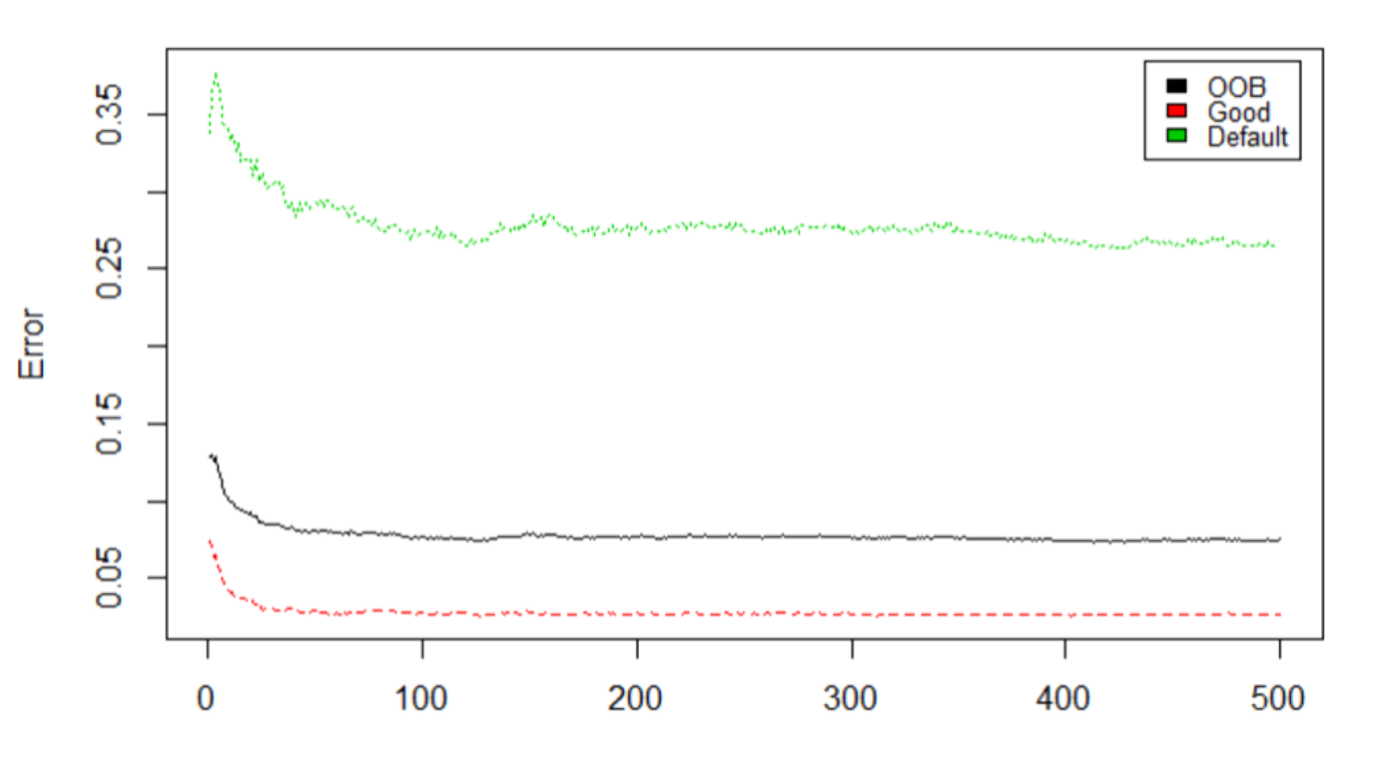
\includegraphics[width=0.7\textwidth]{figure.png}
\caption{A plot with three decaying traces.
Decaying errors are nice
\label{fig:figure}
}
\end{figure}

\section{Theorem environments}

Let's start with something easy:

\begin{thm}[Pythagoras’s Theorem]\label{thm:pythagoras} 

Given a right triangle with hypotenuse $c$, we have
$$
  c^2 = a^2 + b^2
$$

\end{thm}

\begin{lem}[Pumping]\label{lem:pumping} 

If it's good, it can be made better, especially in Computer Science.

\end{lem}

As we see in \cref{thm:pythagoras}, triangles are cool and can be made better with \cref{lem:pumping}.

\printbibliography
\end{document}
